\section{Vectors}
\label{sec:vectors}
Row vectors are fun targets for the \svdl. It's very easy to visualize the domain and codomain.

%%
\subsection{\vv s}
Consider the \vv \ below:
\begin{equation}
  v=\mat{c}{1\\\frac{1}{2}}.
  \label{eq:cases:2v}
\end{equation}
Hopefully the rank of the system is obvious:
\begin{equation}
  \rho = \min\lst{m,n}= \min\lst{2,1} = 1
\end{equation}

The decomposition will have these form factors
\begin{equation}
  \begin{array}{ccccc}
  \A{} &=& \Y{} & \sig{} & \X{T}\\
  \by{m}{n}&=&\paren{\by{m}{m}}&\paren{\by{m}{n}}&\paren{\by{n}{n}}\\
  \by{2}{1}&=&\paren{\by{2}{2}}&\paren{\by{2}{1}}&\paren{\by{1}{1}},
  \end{array}
\end{equation}
as depicted below:
\begin{figure}[htbp] %  figure placement: here, top, bottom, or page
   \centering
   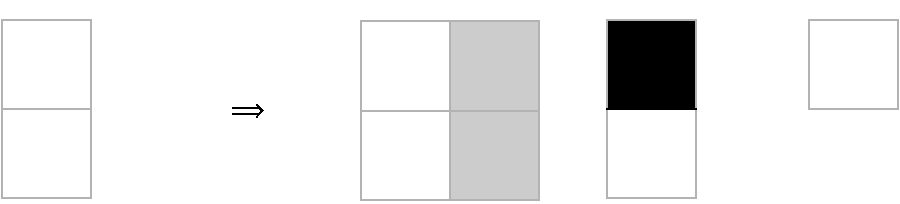
\includegraphics[ width = 4in ]{pdf/more_examples/svd_02_01_01} 
%  ` \caption{example caption}
   \label{fig:examples:21}
\end{figure}

The $\X{}$ matrix is trivial. Since it must be unitary the magnitude is one:
\begin{equation}
  \X{}= \mat{c}{1}.
\end{equation}
The lone singular value is the scale factor $r=\sqrt{2^{2}+\frac{1}{2}^{2}}$ which is the length of the vector:
\begin{equation}
  \sig{} = \mat{c}{\frac{\sqrt{5}}{2}\\0}.
\end{equation}
  For the codomain matrix we start with the image and normalize the column vector:
\begin{equation}
  \Y{}=\mat{cc}{c_{1}&c_{2}}, \qquad c_{1}=\frac{\sqrt{5}}{2}\mat{c}{2\\1}.
\end{equation}
The only quantity missing now is the null space vector $c_{2}$. Pick an orthogonal complement to $c_{1}$ and the codomain basis matrix is
\begin{equation}
  \Y{}=\frac{1}{\sqrt{5}}\mat{rr}{2&1\\1&-2}.
\end{equation}
The \svdl \ is then
\begin{equation}
  \begin{split}
    \svda{T}\\
    \mat{c}{1\\\frac{1}{2}} &= \frac{1}{\sqrt{5}}
    \mat{rr}{2&-1\\1&2}
    \mat{c}{\frac{\sqrt{5}}{2}\\0}
    \mat{c}{1}.
  \end{split}
  \label{eq:cases:2vdecomp}
\end{equation}

%%
\subsection{\vvv s}
Consider this \vvv:
\begin{equation}
  v = \mat{r}{1\\2\\-2}.
\end{equation}
The decomposition will have the shapes given by this
\begin{equation}
  \begin{array}{ccccc}
  \A{} &=& \Y{} & \sig{} & \X{T}\\
  \by{m}{n}&=&\paren{\by{m}{m}}&\paren{\by{m}{n}}&\paren{\by{n}{n}}\\
  \by{3}{1}&=&\paren{\by{3}{1}}&\paren{\by{3}{1}}&\paren{\by{1}{1}},
  \end{array}
\end{equation}
as shown here:
\begin{figure}[htbp] %  figure placement: here, top, bottom, or page
   \centering
   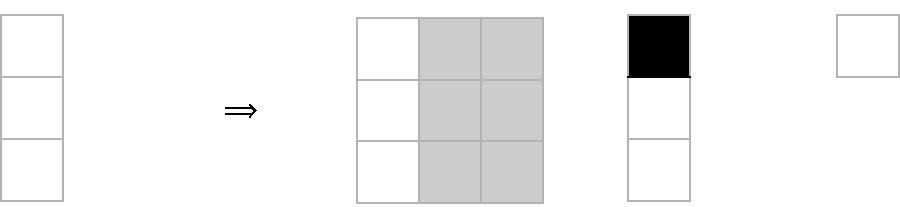
\includegraphics[ width = 4in ]{pdf/more_examples/svd_03_01_01} 
%   \caption{example caption}
   \label{fig:examples:31}
\end{figure}

We can use this vector to seed the codomain matrix:
\begin{equation}
  \Y{}_{*,1} = \frac{1}{3}\mat{r}{1\\2\\-2}.
\end{equation}
This leaves the null space vectors. A first candidate is 
\begin{equation}
  \Y{}_{*,2} = \frac{1}{\sqrt{2}}\mat{r}{0\\1\\1}.
\end{equation}
Using an inspection-based algorithm we can pick a vector like
\begin{equation}
  \Y{}_{*,3} = \frac{1}{\sqrt{18}}\mat{r}{4\\-1\\1}.
\end{equation}
The lone singular value is the length of the vector. The \svdl \ becomes
\begin{equation}
  \begin{split}
    \svda{T}\\
    \mat{r}{1\\2\\-2} &=
    \left[
\begin{array}{ r >{\columncolor{ltgray}}r >{\columncolor{ltgray}}r }
  \frac{1}{3} & 0 & \frac{4}{ \sqrt{18} } \\[5pt]
  \frac{2}{3} & \frac{1}{\sqrt{2}} & -\frac{1}{ \sqrt{18} } \\[5pt]
 -\frac{2}{3} & \frac{1}{\sqrt{2}} &  \frac{1}{ \sqrt{18} }
\end{array}
\right] 
    \left[
\begin{array}{c}
 3 \\ \hline
 0 \\
 0
\end{array}
\right]
  \mat{c}{1}.
  \end{split}
\end{equation}

The shortcut won't work. 
\begin{equation}
  v = \mat{c}{\sin\theta \\ 0 \\ \cos\theta}.
\end{equation}

\begin{equation}
  \begin{split}
    \W{y} = v v^{\mathrm{T}} &= \mat{c}{\sin\theta \\ 0 \\ \cos\theta}\mat{ccc}{\sin\theta & 0 & \cos\theta}\\
    &= \mat{ccc}{\sin^{2}\theta & 0 & \sin\theta \cos\theta\\ 0 & 0 & 0 \\ \sin\theta \cos\theta & 0 & \cos^{2}\theta}
  \end{split}
\end{equation}


Characteristic polynomial
Use cofactor expansion to compute the determinant
\begin{equation}
  \begin{split}
    p(\lambda) &= \det \paren{\W{y} - \lambda \I{3}}\\ &= 
    \det\mat{c|r|c}{\sin^{2}\theta - \lambda & 0 & \sin\theta \cos\theta\\\hline 0 & - \lambda & 0 \\ \sin\theta \cos\theta & 0 & \cos^{2}\theta- \lambda} \\
    &= \paren{\sin^{2}\theta - \lambda}\det\mat{cc}{-\lambda & 0 \\ 0 & \cos^{2}\theta- \lambda}\\ & \quad- 0 \det\mat{cc}{0 & 0 \\ \sin\theta \cos\theta & \cos^{2}\theta- \lambda}\\
     & \quad + \paren{\cos^{2}\theta - \lambda}\det\mat{cc}{0 & -\lambda \\ \sin\theta \cos\theta & 0}\\
  \end{split}
\end{equation}

The roots of the characteristic polynomial are the eigenvalues
\begin{equation}
  p(\lambda) = \lambda^{2}\paren{\lambda-1} = 0
\end{equation}
leads to the spectrum
\begin{equation}
  \lambda\paren{\W{y}} = \lst{1,0,0}.
\end{equation}
Therefore there is one singular value, 
\begin{equation}
  \sigma_{1} = 1.
\end{equation}
The eigenvector solves
\begin{equation}
  \begin{split}
    \W{y}u &= \lambda u\\
    \mat{ccc}{\sin^{2}\theta & 0 & \sin\theta \cos\theta\\ 0 & 0 & 0 \\ \sin\theta \cos\theta & 0 & \cos^{2}\theta} \mat{c}{u_{1} \\ 0 \\ u_{3}} & = \mat{c}{u_{1} \\ 0 \\ u_{3}}
  \end{split}
\end{equation}
This reduces to the system
\begin{equation}
\mat{cc}
{\sin^{2}\theta & \sin\theta \cos\theta\\
 \sin\theta \cos\theta & \cos^{2}\theta}
\mat{c}{u_{1} \\ u_{3}} = \mat{c}{u_{1} \\ u_{3}}
\end{equation}



%%
\subsection{$10-$vectors}
You can quickly verify that
\begin{equation}
  \begin{split}
    \svda{T}\\
    \mat{r}{1\\0\\0\\0\\0\\0\\0\\0\\0\\0} &=
    \left[
\begin{array}{ r >{\columncolor{ltgray}}r >{\columncolor{ltgray}}r >{\columncolor{ltgray}}r >{\columncolor{ltgray}}r >{\columncolor{ltgray}}r >{\columncolor{ltgray}}r >{\columncolor{ltgray}}r >{\columncolor{ltgray}}r >{\columncolor{ltgray}}r }
  1 & 0 & 0 & 0 & 0 & 0 & 0 & 0 & 0 & 0 \\
  0 & 1 & 0 & 0 & 0 & 0 & 0 & 0 & 0 & 0 \\
  0 & 0 & 1 & 0 & 0 & 0 & 0 & 0 & 0 & 0 \\
  0 & 0 & 0 & 1 & 0 & 0 & 0 & 0 & 0 & 0 \\
  0 & 0 & 0 & 0 & 1 & 0 & 0 & 0 & 0 & 0 \\
  0 & 0 & 0 & 0 & 0 & 1 & 0 & 0 & 0 & 0 \\
  0 & 0 & 0 & 0 & 0 & 0 & 1 & 0 & 0 & 0 \\
  0 & 0 & 0 & 0 & 0 & 0 & 0 & 1 & 0 & 0 \\
  0 & 0 & 0 & 0 & 0 & 0 & 0 & 0 & 1 & 0 \\
  0 & 0 & 0 & 0 & 0 & 0 & 0 & 0 & 0 & 1 \\
\end{array}
\right] 
    \left[
\begin{array}{c}
 1 \\ \hline
 0 \\
 0 \\
 0 \\
 0 \\
 0 \\
 0 \\
 0 \\
 0 \\
 0
\end{array}
\right]
  \mat{c}{1}.
  \end{split}
\end{equation}

This is such a simple exercise because the column vectors are already unit vectors.

A Givens rotation by an angle $\theta$ in the $4-8$ plane does not affect the decomposition because the codomain matrix $\Y{}$ is still orthogonal
\begin{equation}
  \Y{'} = 
      \left[
\begin{array}{ c >{\columncolor{ltgray}}c >{\columncolor{ltgray}}c >{\columncolor{ltgray}}c >{\columncolor{ltgray}}c >{\columncolor{ltgray}}c >{\columncolor{ltgray}}c >{\columncolor{ltgray}}c >{\columncolor{ltgray}}c >{\columncolor{ltgray}}c }
  1 & 0 & 0 & 0 & 0 & 0 & 0 & 0 & 0 & 0 \\
  0 & 1 & 0 & 0 & 0 & 0 & 0 & 0 & 0 & 0 \\
  0 & 0 & 1 & 0 & 0 & 0 & 0 & 0 & 0 & 0 \\
  0 & 0 & 0 & \cos \theta & 0 & 0 & 0 & -\sin \theta & 0 & 0 \\
  0 & 0 & 0 & 0 & 1 & 0 & 0 & 0 & 0 & 0 \\
  0 & 0 & 0 & 0 & 0 & 1 & 0 & 0 & 0 & 0 \\
  0 & 0 & 0 & 0 & 0 & 0 & 1 & 0 & 0 & 0 \\
  0 & 0 & 0 & \sin \theta & 0 & 0 & 0 & \cos \theta & 0 & 0 \\
  0 & 0 & 0 & 0 & 0 & 0 & 0 & 0 & 1 & 0 \\
  0 & 0 & 0 & 0 & 0 & 0 & 0 & 0 & 0 & 1 \\
\end{array}
\right] 
\end{equation}

Yet another rotation 1-9:
\begin{equation}
  \Y{'} = 
      \left[
\begin{array}{ c >{\columncolor{ltgray}}c >{\columncolor{ltgray}}c >{\columncolor{ltgray}}c >{\columncolor{ltgray}}c >{\columncolor{ltgray}}c >{\columncolor{ltgray}}c >{\columncolor{ltgray}}c >{\columncolor{ltgray}}c >{\columncolor{ltgray}}c }
  \cos \phi & 0 & 0 & 0 & 0 & 0 & 0 & 0 & -\sin \phi & 0 \\
  0 & 1 & 0 & 0 & 0 & 0 & 0 & 0 & 0 & 0 \\
  0 & 0 & 1 & 0 & 0 & 0 & 0 & 0 & 0 & 0 \\
  0 & 0 & 0 & \cos \theta & 0 & 0 & 0 & -\sin \theta & 0 & 0 \\
  0 & 0 & 0 & 0 & 1 & 0 & 0 & 0 & 0 & 0 \\
  0 & 0 & 0 & 0 & 0 & 1 & 0 & 0 & 0 & 0 \\
  0 & 0 & 0 & 0 & 0 & 0 & 1 & 0 & 0 & 0 \\
  0 & 0 & 0 & \sin \theta & 0 & 0 & 0 & \cos \theta & 0 & 0 \\
  \sin \phi & 0 & 0 & 0 & 0 & 0 & 0 & 0 & \cos \phi & 0 \\
  0 & 0 & 0 & 0 & 0 & 0 & 0 & 0 & 0 & 1 \\
\end{array}
\right] 
\end{equation}


\endinput